\subsection{[Aatos] NN analysis}

{\tt root\_v5.21.06}
Compiled with {\tt make -j2} option used for dual CPU machines.

\subsubsection{Default variables, default cuts}
\scriptsize
\begin{verbatim}

\end{verbatim}
\normalsize

(See Figs.\ref{fig:variables_c1}),
 
\begin{figure}[h]
 \begin{minipage}{7.0cm}
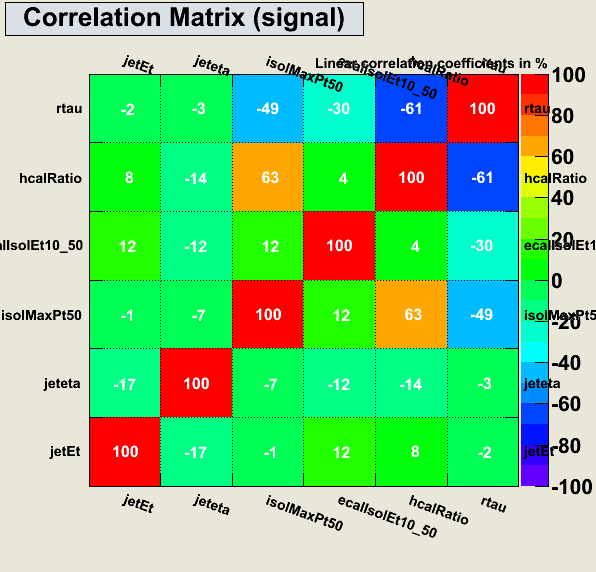
\includegraphics[width=1.0\textwidth]{images/ahCorrelationMatrixS.png}
\end{minipage}
 \hfill
\begin{minipage}{7.0cm}
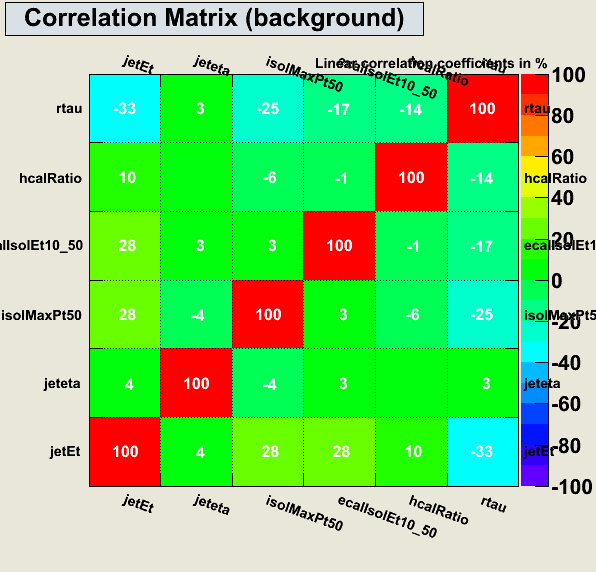
\includegraphics[width=1.0\textwidth]{images/ahCorrelationMatrixB.png}
\end{minipage}
\begin{minipage}{3.0cm}
\caption{Right: Variable correlation matrix for signal Right: Variable correlation matrix for background}
\end{minipage}
\label{fig:ahCorrelationMatrix}
\end{figure}


\begin{figure}[h]
\begin{center}
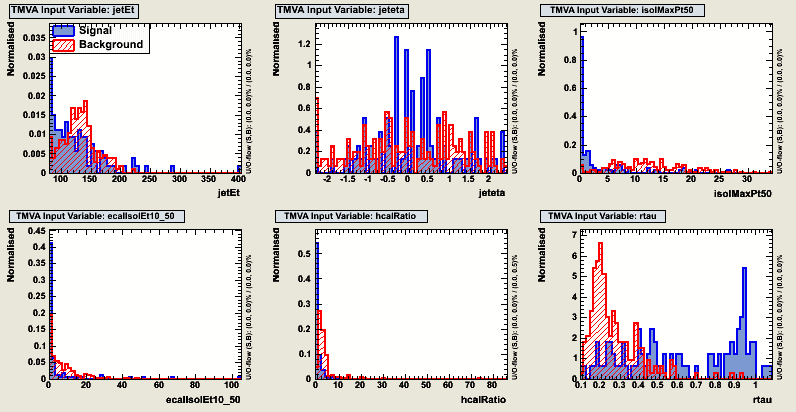
\includegraphics[width=1.0\textwidth]{images/ahVariables_c1.png}
\caption{Variables used in the analysis. Notice log transformations used for some of the variables.}
\label{fig:variables_c1}
\end{center}
\end{figure}

 
\begin{figure}[h]
 \begin{minipage}{7.0cm}
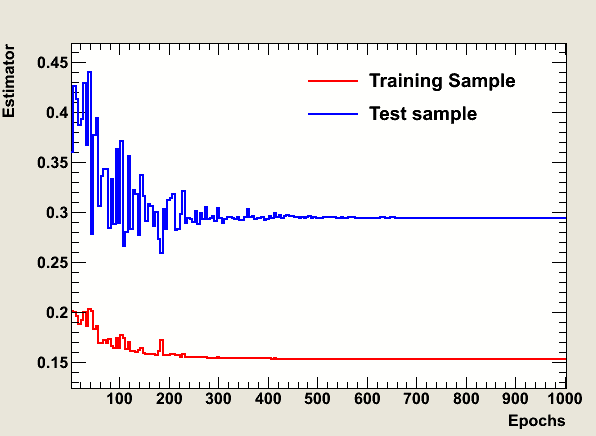
\includegraphics[width=1.0\textwidth]{images/ahAnnconvergencetest.png}
\end{minipage}
 \hfill
\begin{minipage}{7.0cm}
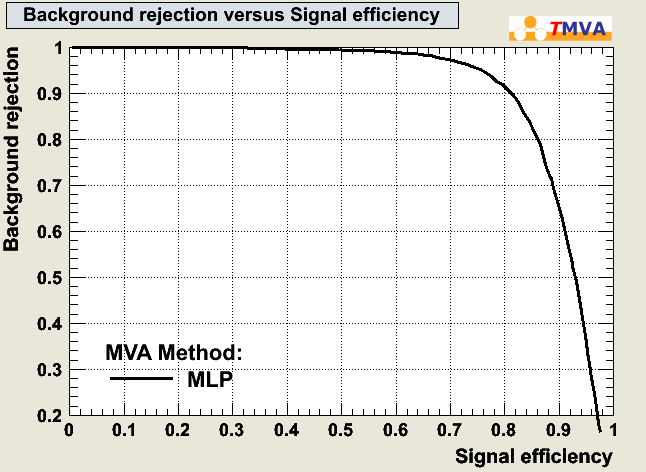
\includegraphics[width=1.0\textwidth]{images/ahRejBvsS.png}
\end{minipage}
\begin{minipage}{3.0cm}
\caption{Left: ANN convergence test. Right: Signal vs. background rejection for ANN classifier.}
\end{minipage}
\label{fig:mlp}
\end{figure}


\clearpage

\begin{figure}[!h]
\begin{center}
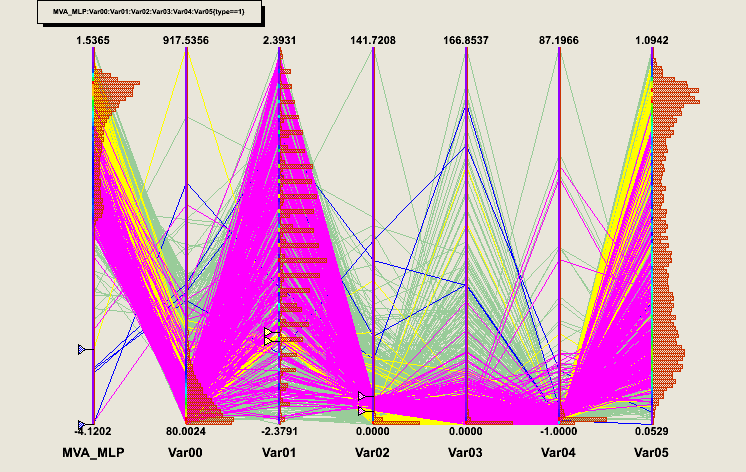
\includegraphics[width=0.6\textwidth]{images/ahParacoor_c0_S.png}
\caption{Parallel coordinates for signal. 
(For more information on parallel coordinates plot see \url{http://en.wikipedia.org/wiki/Parallel_coordinates}.)}
\label{fig:ahParacoor_c0_S}
\end{center}
\end{figure}
\begin{figure}[!h]
\begin{center}
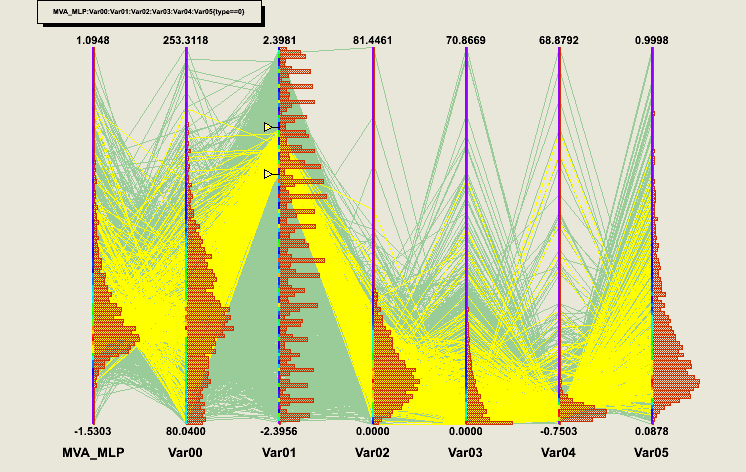
\includegraphics[width=0.6\textwidth]{images/ahParacoor_c0_B.png}
\caption{Parallel coordinates for background}
\label{fig:ahParacoor_c0_B}
\end{center}
\end{figure}

\clearpage

 
\begin{figure}[h]
 \begin{minipage}{7.0cm}
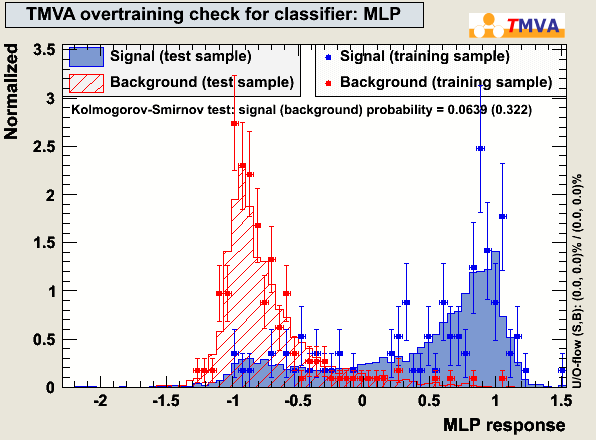
\includegraphics[width=1.0\textwidth]{images/ahOvertrain_MLP.png}
\end{minipage}
\hfill
\begin{minipage}{7.0cm}
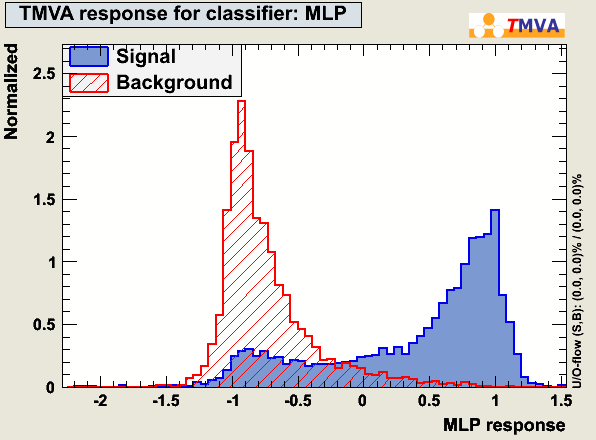
\includegraphics[width=1.0\textwidth]{images/ahMva_MLP.png}
\end{minipage}
\begin{minipage}{3.0cm}
\scriptsize
\caption{Left: Overtrain test. Right: MLP output for test data.}
\normalsize
\end{minipage}
\label{fig:mlp}
\end{figure}



%\subsection{chep09tmva\_aatos.C}
\lstset{
language=C++,
numbers=left,
stepnumber=2,
caption={\tt code/chep09tmva\_aatos.C},
label=chep09tmva_aatos
}
%\lstinputlisting{code/chep09tmva_aatos.C}

%\subsection{chep09tmva.cc}
\lstset{
language=C++,
numbers=left,
stepnumber=2,
caption={\tt code/chep09tmva.cc},
label=chep09tmvacc
}
%\lstinputlisting{code/chep09tmva.cc}


%git fetch pekka
%git merge pekka/master
%gitk 
%(modify)
%git diff
%git status
%git commit -a -m 'comment'  (add all changes)
%(modify)
%git diff
%git commit -a -m 'comment'  

%gitk 
%git revert HEAD  (in case of bad commit this reverses it)

%git push 

%make release


%.gitconfig}:
%
%[user]
%	email = aatos.heikkinen@cern.ch
%[color]
%       ui = auto






